
%(BEGIN_QUESTION)
% Copyright 2006, Tony R. Kuphaldt, released under the Creative Commons Attribution License (v 1.0)
% This means you may do almost anything with this work of mine, so long as you give me proper credit

Suppose we have a condition where the PV signal is 5.8 PSI and the SP signal is 7.2 PSI.  Determine the pressure inside the reset bellows at the moment when the output signal is 11.3 PSI, and determine whether the output pressure will be {\it rising} or {\it falling}:

$$\includegraphics[width=15.5cm]{i01633x01.eps}$$

Assume all four bellows are identical in dimensions and construction, and that the fulcrum is placed exactly mid-way between the two sets of bellows.

\vfil 

\underbar{file i01633}
\eject
%(END_QUESTION)





%(BEGIN_ANSWER)

This is a graded question -- no answers or hints given!

%(END_ANSWER)





%(BEGIN_NOTES)

Reset bellows pressure = 12.7 PSI

\vskip 10pt

Output pressure will be {\it falling} over time.

\vskip 10pt

A general principle of all force-balance mechanisms is that -- quite obviously -- all forces must be balanced.  If the setpoint signal is greater than the PV signal (resultant force {\it down} on the right-hand side of the lever, creating a clockwise torque), then the reset bellows pressure must be greater than the output bellows pressure (resultant force {\it down} on the lever, creating a counter-clockwise torque).  With all bellows equal-size and equidistant from the fulcrum, we may conclude that the imbalance of signal pressures on the left-hand side must be the same as the imbalance of pressures on the right-hand side.  With SP 1.4 PSI greater than PV, the reset bellows pressure must also be 1.4 PSI greater than the output bellows, and so the reset bellows pressure must be 12.7 PSI.

As to the direction of pressure change in the reset bellows, we may apply two completely different principles to arrive at the same result.  One principle is that the reset action should be ``winding'' in the direction appropriate to the action of the controller.  In this case, we can see that the controller is direct-acting, and so a condition where PV $<$ SP should result in the output pressure {\it decreasing}, which must mean the reset bellows pressure is decreasing as well.  A different principle we may apply is the direction of fluid motion through a restriction given a known pressure drop: the reset adjust valve sees a greater pressure on its top side (reset bellows side) than on its bottom side (output), which tells us the air flow through it will be down, emptying air from the reset bellows (imagine a resistor passing conventional-flow current downward because the potential is greater (+) on the top than on the bottom).

%INDEX% Control, proportional + integral: pneumatic force-balance controller

%(END_NOTES)


